\documentclass[10pt,twocolumn]{article}

% use the oxycomps style file
\usepackage{oxycomps}

% usage: \fixme[comments describing issue]{text to be fixed}
% define \fixme as not doing anything special
\newcommand{\fixme}[2][]{#2}
% overwrite it so it shows up as red
\renewcommand{\fixme}[2][]{\textcolor{red}{#2}}
% overwrite it again so related text shows as footnotes
%\renewcommand{\fixme}[2][]{\textcolor{red}{#2\footnote{#1}}}

% read references.bib for the bibtex data
\bibliography{references}

% include metadata in the generated pdf file
\pdfinfo{
    /Title (The Occidental Computer Science Comprehensive Project: Goals, Timeline, Format, and Advice)
    /Author (Justin Li)
}

% set the title and author information
\title{The Occidental Computer Science Comprehensive Project: \\ Goals, Timeline, Format, and Advice}
\author{Justin Li}
\affiliation{Occidental College}
\email{justinnhli@oxy.edu}

\begin{document}

\maketitle

\section{Introduction}

This document serves describes the Oxy CS Comps process.
The first section describes the timeline of comps, as well as the main requirements of a comps project.
Since one of the main deliverable is a final paper, there is then an interlude on {\LaTeX}, which you will use to write the paper.
This document then goes into the sections of that final paper and what is expected of it.
We conclude with some miscellaneous tips for successfully completing comps.

\section{Computer Science Comps}

Occidental's ``Comprehensive Requirement'' is a graduation requirement that serves two goals: ``to provide an opportunity for senior students to synthesize the essential[s] [...] of their academic field'', and ``to provide an opportunity for students to demonstrate competence in their field'' \cite{OccidentalComps}.
For computer science, the breadth of the field means that comps leans heavily towards the second goal: most CS comps are large coding projects that showcase what a student has learned in their four years at Oxy.
In that sense, a CS comps project is more like a Studio Arts comps project: you could draw from multiple subfields or focus on just one, but the essence is to take on a complex project of your choice while situating it within the methods of CS.

\subsection{Timeline}

Since comps is a significant undertaking, the CS major curriculum has two courses to support comps projects.
Most students will take CS Junior Seminar in the spring of their junior year, then take CS Senior Seminar in the fall of their senior year.
One of the main goals of Junior Seminar is to prepare students for their comps project, including selecting a topic, exploring the literature, and writing a detailed proposal of what they will do.
The entirety of Senior Seminar is dedicated to students completing their comps; however, it is necessary to separate the Senior Seminar course from the comps graduation requirement.
Senior Seminar is a required course for the CS major, and it concludes at the end of the fall semester with a grade.
Comps, on the other hand, is an Oxy graduation requirement, and concludes at the end of the senior year with either ``fail'', ``pass'', or ``pass with distinction'' \cite{OccidentalComps}.
While the sole purpose of Senior Seminar is to support students working on comps, it is possible for a student to complete the \textit{course} without completing the \textit{graduation requirement}.
This could occur, for example, if the student ran out of time to finish the project, but submitted all the assignments for Senior Seminar.
In that case, the student will continue working in the spring senior semester to complete their comps, until they have a ``pass'' or ``pass with distinction'' result.
A summary of this timeline can be found in Table \ref{tbl:timeline}.

\begin{table}
    \footnotesize
    \begin{tabular}{r|cl}
        \textbf{Semester}       &  \textbf{Course}  &  \textbf{Deliverable(s)}          \\
        \hline \\
        \textbf{Junior Spring}  &  COMP 390         &  Comps proposal; Tutorial report  \\
        \textbf{Summer}         &  -                &  Additional research              \\
        \textbf{Senior Fall}    &  COMP 490         &  Comps final paper; Code repo     \\
        \textbf{Senior Spring}  &  -                &  Revisions; Honors                \\
    \end{tabular}
    \caption{Timeline summary for comps.}
    \label{tbl:timeline}
\end{table}

\subsection{Deliverables}

The two main deliverables for CS comps is the code from the project, submitted together with its documentation as a GitHub link, and a paper about the project.
While the code component is straightforward and uncontroversial, some students may chafe against the idea of a paper.
Contrary to popular believe, the job of a software engineer does not only involve writing code.
It also requires a large amount of written communication, such as tickets for bugs reports, proposals for new features and why it will improve the product, comments on why a class is necessary or how a function works, and documentation of the system architecture.
As software engineers rise from junior to senior positions, these responsibilities only increase.
It is often lamented that not enough engineers know how to write \cite{Mei2018WhyDevelopersShould,Alton2020WhyEveryDeveloper}, which is why Google has created courses on technical writing \cite{GoogleTechnicalWriting}, and ``soft skills'' are routinely touted as necessary for software developers \cite{Indeed202111ImportantSoft}.

\begin{comment}
    Why a paper?
    Goals for the paper
\end{comment}

Given these goals, the final paper should be written for an advanced CS undergraduate: someone who has finished Math Foundations, Data Structures, and Computer Organization, but may not have taken the appropriate upper-level courses.
The paper does not need to explain everything, but should provide enough relevant details so the average reader can understand your results; a walkthrough of the sections of the paper can be found in Section \ref{sec:paper}.
The paper will be written in LaTeX, to make all final papers uniform in style and to allow for psuedocode and mathematical equations; a template will be provided and required.
To ensure there is sufficient context and detail, the paper should be about seven pages in length (excluding figures, tables, code, and references).
The target audience for the paper is other computer science majors in their final year of college, but who may not have taken the same electives that you have.
That is, you should assume that they have working knowledge of data structures, discrete math, and computer systems, but not necessarily any knowledge of artificial intelligence, machine learning, databases, or other more advanced topics.

The other major deliverable is the code, which should be made available on a public GitHub repository.
Accompanying the code should be two pieces of documentation, both included in a \texttt{README.md}.
First, there should be instructions for how to run the code, which should including how to find and install necessary software and packages, how to find and download relevant datasets, and what other requirements (hardware, spatial needs for VR, etc.) are needed.
This should be written for an audience who is interested in reproducing your work and verifying your results.
Second, there should be a brief overview of how the code is organized, including the major components that exist and the content and format of the data that is passed between them.
This should be written for someone who is interested in extending your project --- say, by tweaking the parameters, or adding new functionality, or applying it to a new context.

More details about both deliverables will be provided in the Junior and Seminar Seminars.

\begin{comment}
    something about non-code projects?
\end{comment}

\subsection{Selecting a Comps Project}

For many students, selecting a topics for comps is a major source of stress.
While this is an important decision, it is also one for which you will receive a lot of support.
Choosing a topic, together with ensuring that you have the relevant background and experience for the project, is a major component of Junior Seminar.
There have also been students who change their project during Senior Seminar, and still finished their comps within the semester; although this is not recommended, this delayed timeline shows how much leeway there is for exploration and backpedaling.

As a rough guide, comps projects should be equivalent to the work of an upper-level CS elective, and should either dive deeply but narrowly into a subfield of CS, or reach broadly across subfields or across disciplines without being too shallow.
The only constraint on the topic is that CS+Math and CS+X students must select a project that fits within their theme, and should check with their academic advisor to make sure this is the case.
Although double majors could do both comps on the same topic, they must have aspects that are unique to each major.
For example, a cognitive science and computer science double major could do both projects around biologically plausible neural networks, but the cognitive science project might be about comparing its activity to real brains, while the CS project might instead focus on its algorithmic performance.
We will spend more time on this in class, but you might consider the following prompts in brainstorming your project:

\begin{itemize}
    \item What topics were you most interested in from your classes? What area of CS would you like to dive deeper into?
    \item Alternately, what topic were you unable to take a class in (either due to full enrollments, or because Oxy doesn't offer it)?
    \item What interdisciplinary topics or CS-adjacent topics would you like to explore?
    \item What projects might be a good showcase of your abilities to potential employers in your desired field?
\end{itemize}

A list of past comps projects can be found online.\footnote{\url{https://www.oxy.edu/academics/areas-study/computer-science/past-senior-comps-projects}}

\section{Interlude: Using \LaTeX}

LaTeX (pronounced \textit{lah-teck} or \textit{lay-teck}), often stylized as {\LaTeX} and written as latex, is a document markup language and typesetting system.
Building on the {\TeX} language created by Donald Knuth in 1978, LaTeX provides additional commands for common document needs such as sections, figures, and bibliographies.
LaTeX is widely used in academia, especially in mathematical fields, due to how easy it is to write mathematical equations and its automatic management of references.
Since it is a markup language, LaTeX source files are written in plain text, which also makes it compatible with version control systems like git.

The most primitive syntax of LaTeX is the \textit{macro} or \textit{command}, which is always written with a backslash followed by the name of the command.
The {\LaTeX} glyph, for example, can be created with the command \texttt{\textbackslash LaTeX}.
Some commands take parameters, which are denoted in braces (e.g., \texttt{\textbackslash usepackage\{biblatex\}} will import the \texttt{biblatex} package), with some commands additionally accepting options in square brackets (e.g., \texttt{\textbackslash usepackage[style=numeric]\{biblatex\}}).
The \texttt{\textbackslash begin} and \texttt{\textbackslash end} commands are special, as they indicate the start and end of an \textit{environment}.
The content of a LaTeX document, for example, is surrounded by \texttt{\textbackslash begin\{document\}} and \texttt{\textbackslash end\{document\}}, indicating the text that should appear in the document.

\begin{figure}
    \centering
    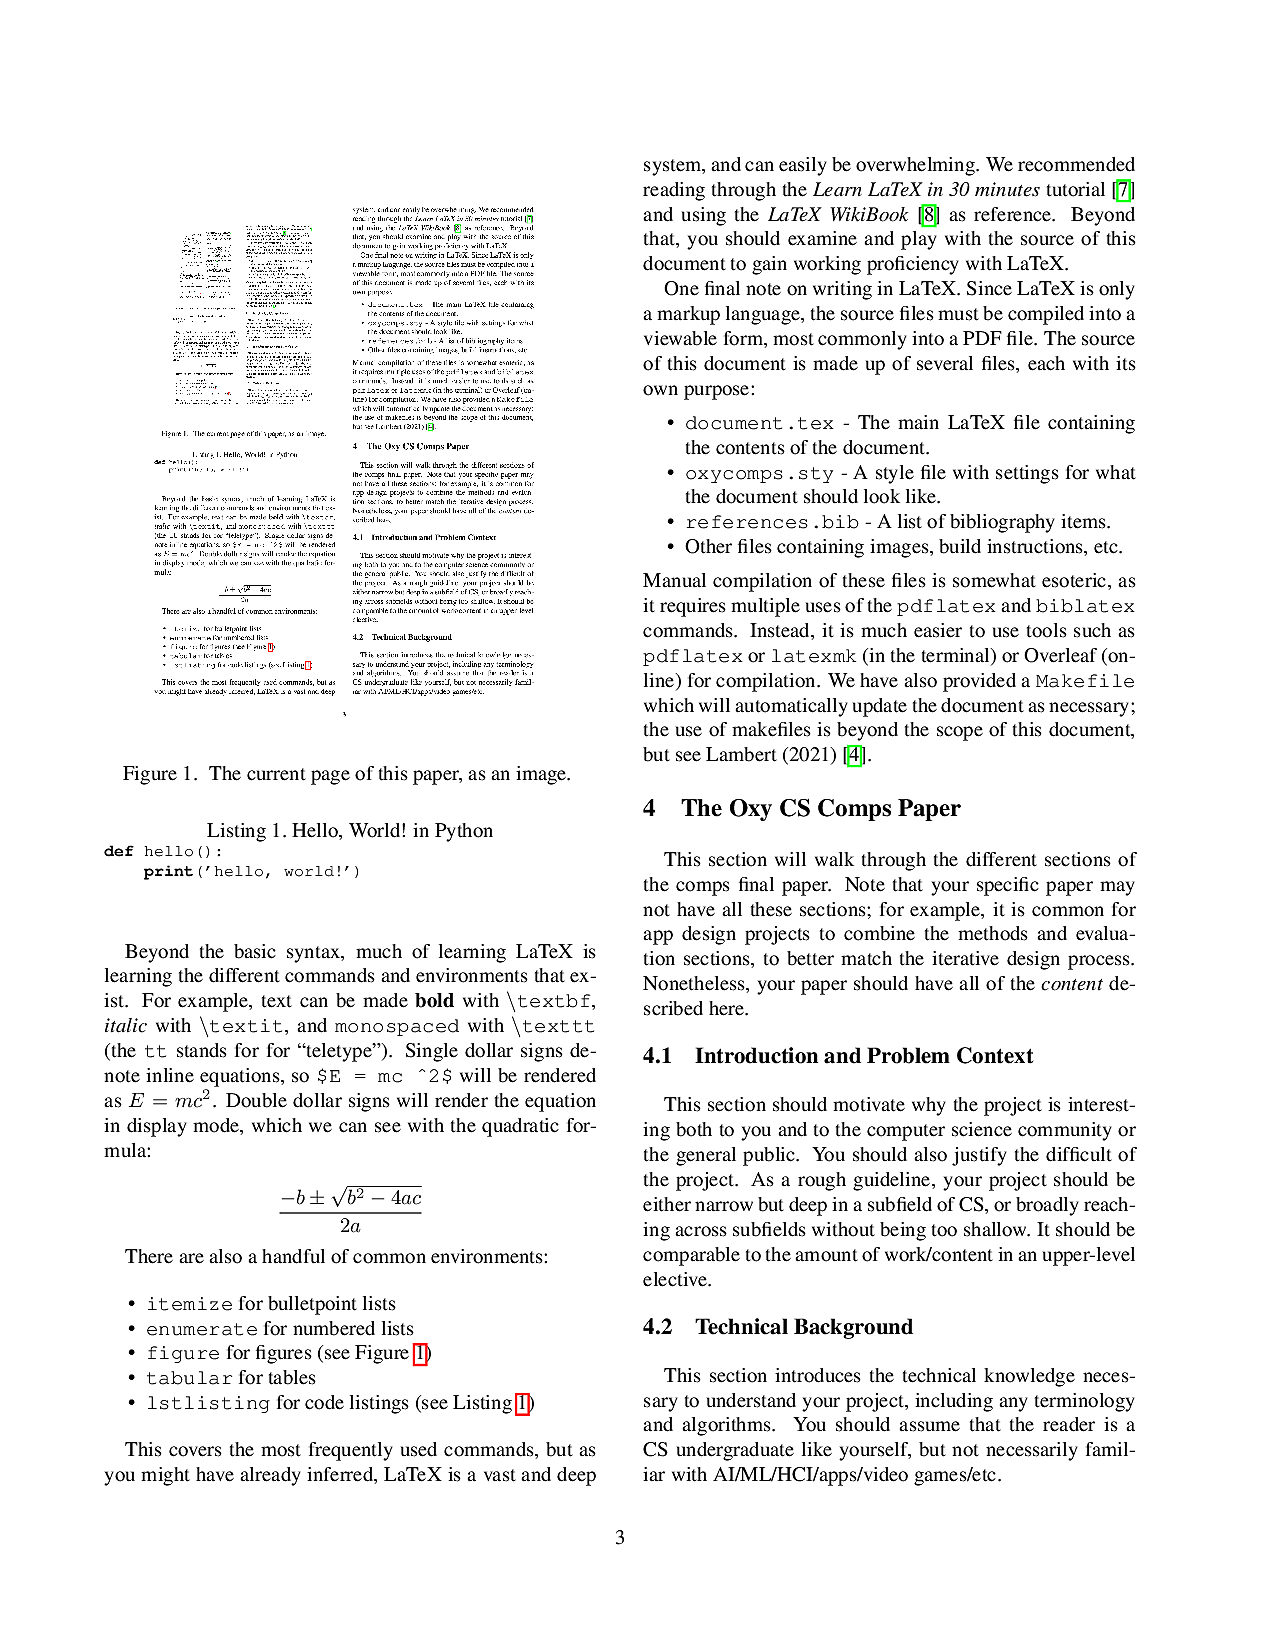
\includegraphics[width=.95\linewidth]{recursion.png}
    \caption{
        The current page of this paper, as an image.
    }
    \label{fig:first-page}
\end{figure}

Beyond the basic syntax, much of learning LaTeX is learning the different commands and environments that exist.
For example, text can be made \textbf{bold} with \texttt{\textbackslash textbf}, \textit{italic} with \texttt{\textbackslash textit}, and \texttt{monospaced} with \texttt{\textbackslash texttt} (the \texttt{tt} stands for for ``teletype'').
Single dollar signs denote inline equations, so \texttt{\$E = mc\textasciicircum 2\$} will be rendered as $E = mc^2$.
Double dollar signs will render the equation in display mode, which we can see with the quadratic formula:

$$\frac{{-b \pm \sqrt {b^2 - 4ac} }}{{2a}}$$

There are also a handful of common environments:

\begin{itemize}
    \item \texttt{itemize} for bulletpoint lists
    \item \texttt{enumerate} for numbered lists
    \item \texttt{figure} for figures (see Figure \ref{fig:first-page})
    \item \texttt{table} and \texttt{tabular} for tables (see Table \ref{tbl:timeline})
    \item \texttt{lstlisting} for code listings (see Listing \ref{lst:python-hello-world})
\end{itemize}

\begin{lstlisting}[
    language=Python,
    caption={Hello, World! in Python},
    label={lst:python-hello-world},
    float
]
def hello():
    print('hello, world!')
\end{lstlisting}

This covers the most frequently used commands, but as you might have already inferred, LaTeX is a vast and deep system, and can easily be overwhelming.
We recommended reading through the \citetitle{Overleaf2021LearnLaTeXIn} tutorial \cite{Overleaf2021LearnLaTeXIn} and using the \citetitle{WikiBook2022LaTeX} \cite{WikiBook2022LaTeX} as reference.
Beyond that, you should examine and play with the source of this document to gain working proficiency with LaTeX.

One final note on writing in LaTeX.
Since LaTeX is only a markup language, the source files must be compiled into a viewable form, most commonly into a PDF file.
The source of this document is made up of several files, each with its own purpose:
\begin{itemize}
    \item \texttt{document.tex} - The main LaTeX file containing the contents of the document.
    \item \texttt{oxycomps.sty} - A style file with settings for what the document should look like.
    \item \texttt{references.bib} - A list of bibliography items.
    \item Other files containing images, build instructions, etc.
\end{itemize}
Manual compilation of these files is somewhat esoteric, as it requires multiple uses of the \texttt{pdflatex} and \texttt{biblatex} commands.
Instead, it is much easier to use tools such as \texttt{pdflatex} or \texttt{latexmk} (in the terminal) or Overleaf (online) for compilation.
We have also provided a \texttt{Makefile} which will automatically update the document as necessary; the use of makefiles is beyond the scope of this document, but see \textcite{Lambert2021MakefileTutorial}.

\begin{comment}
No definition citations, unless the term itself is in dispute
Separate problem background from technical background
    Unclear if games and apps require much technical background
    The general structure of the framework might be better suited for the Architecture Overview section
        Eg. Flask uses decorators to associate functions with URLs
        Eg. Unity has scripts associated with objects and specific triggers, such as walking into an area, pressing a button, etc.
    Maybe a better name is "algorithmic background"?
        Should explore what does and doesn't count
            All ML counts
            App and game frameworks do not
        Framework vs. library?
            I like the idea of [inversion of control](https://martinfowler.com/bliki/InversionOfControl.html), but that may be too abstract for students to understand
        Heuristic: is understanding that system necessary to understand the results?
            Ie. How Flask or Unity works doesn't influence whether the app/game is useful/fun/engaging
            But how (say) linear regression works is highly relevant for why the results match/don't match the actual values
\end{comment}

\section{The Oxy CS Comps Paper}
\label{sec:paper}

This section will walk through the different sections of the comps final paper.
Note that your specific paper may not have all these sections; for example, it is common for app design projects to combine the methods and evaluation sections, to better match the iterative design process.
Nonetheless, your paper should have all of the \textit{content} described here.

\subsection{Introduction and Problem Context}

This section should motivate why the project is interesting both to you and to the computer science community or the general public.
You should also justify the difficult of the project.
As a rough guideline, your project should be either narrow but deep in a subfield of CS, or broadly reaching across subfields without being too shallow.
It should be comparable to the amount of work/content in an upper-level elective.

\subsection{Technical Background}

This section introduces the technical knowledge necessary to understand your project, including any terminology and algorithms.
You should assume that the reader is a CS undergraduate like yourself, but not necessarily familiar with AI/ML/HCI/apps/video games/etc.

\subsection{Prior Work}

This section describes of related and/or existing work.
This could be scientific or scholarly, but may also be a survey of existing products/games.
The goal of this section is to put your project in the context of what has already been done.

\subsection{Methods}

This section describes what exactly you will be working on.
What are you building? How will it combine/incorporate ideas from the literature? Be specific about what you will be doing: talk about the specific algorithm you will implement/use, the specific dataset/platform/API, and what the outcome of your project will look like.
All of these decisions should be justified as well.

\subsection{Evaluation Metrics}

This section describes how you will evaluate your project.
What will you be measuring, and how will you measure it?
You might think about what would result in an F, a C, or an A for comps.
Alternately, think about what are the minimal requirements for passing the class, what you might do if you had more time and resources, and what the best case scenario would be if everything went swimmingly.

\subsection{Evaluation Results and Discussion}

limitations

\subsection{Ethical Considerations}

Are there any ethical concerns that might arise from your project?
You might think about whether your project perpetuates societal inequity (or could be used by others to do so), whether the data/platforms you are using is collected with informed consent and free of bias, and whether you might be subject to technological solutionism instead of working support/better the public infrastructure.
Include a discussion of how you plan to mitigate these issues in your project.

\subsection{Future Work, and Conclusion}

\subsection{Timeline}

A timeline of major milestones, with specific items to be completed by specific dates/months.
Note that this timeline must start over the summer; otherwise you will unlikely have enough time to complete a project of the expected scope.
As part of the discussion around your timeline, talk about what you already know that would help you with the project, and what you expect to have to learn to be successful.
Include programming languages, technical concepts, as well as processes (e.g., user testing).

\subsection{Code Documentation}

This section will demonstrate that you have thought through the basics of how your code will work. You should include a diagram of the overall data flow of your program, including what the inputs and outputs of each component will be, and how they will be represented.

\subsection{Appendices}

\section{Tips and Advice}

\printbibliography

\end{document}
